\section{Information about missing data}
We have a total of $2.1\%$ of missing values but this number is overestimated because the binary indicators are taken into account. The real ratio is $1.7\%$
without this indicators.
The missing values are due to hardware problems related to the measuring instruments
and to the fact that the data was collected in a real environment.

\begin{figure}[H]
  \centering
  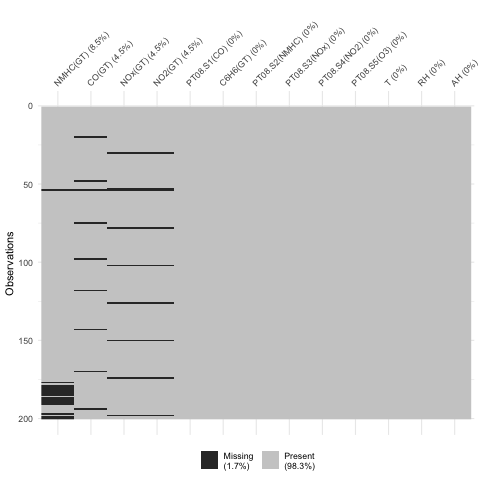
\includegraphics[width=0.5\textwidth]{figs/missing_values.png}
  \caption{Missing data}
  \label{fig:missing_data}
\end{figure}

\begin{figure}[H]
  \centering
  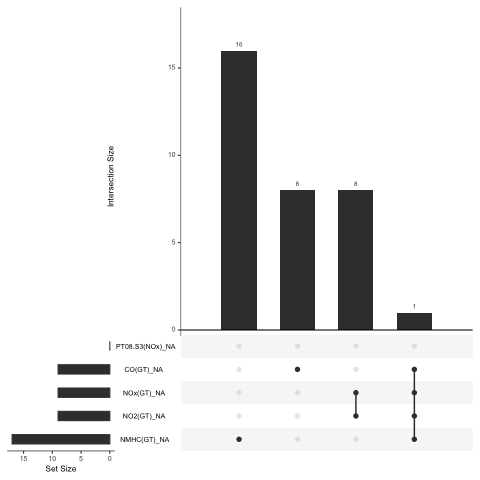
\includegraphics[width=0.5\textwidth]{figs/missing_values_heatmap.png}
  \caption{Missing data heatmap}
  \label{fig:missing_data_heatmap}
\end{figure}

To handle the missing values we will use for the rest of the project the complete case strategy.
Indeed, replacing missing data by the mean would not be a good idea because it would change the correlation structure of the data which is important for the next steps.
We only have 33 lines with missing values so we can afford to remove them keeping the ratio $\frac{n}{p} > 5$ as we have a total of 


